%%%%%%%%%%%%%%%%%%%%%%%%%%%%%%%%%%%%%%%%%%%%%%%%%%%%%%%%%%%%%%%%
\begin{frame}[fragile]\frametitle{}
\begin{center}
{\Large Zenoga}


{\tiny (Based on ``Zen Yoga'' by P J Saher And Deep Knowledge YouTube Channel by Dr Ashish Shukla)}
\end{center}
\end{frame}


%%%%%%%%%%%%%%%%%%%%%%%%%%%%%%%%%%%%%%%%%%%%%%%%%%%%%%%%%%%%%%%%
\begin{frame}[fragile]
\frametitle{Prelude}

\begin{columns}[T] % align columns
\begin{column}{.48\textwidth}
\begin{itemize}
\item Mind is divided into 4 sections
	\begin{itemize}
	\item Section 1 : Brain
	\item Section 2 a: RAS
	\item Section 2 b:
	\item Section 3
	\item Section 4
	\end{itemize}
\item Lower Dimension: 1, 2a
\item Higher Dimension: 2b, 3, 4
\end{itemize}
\end{column}%
\hfill%
\begin{column}{.48\textwidth}
 \begin{center}
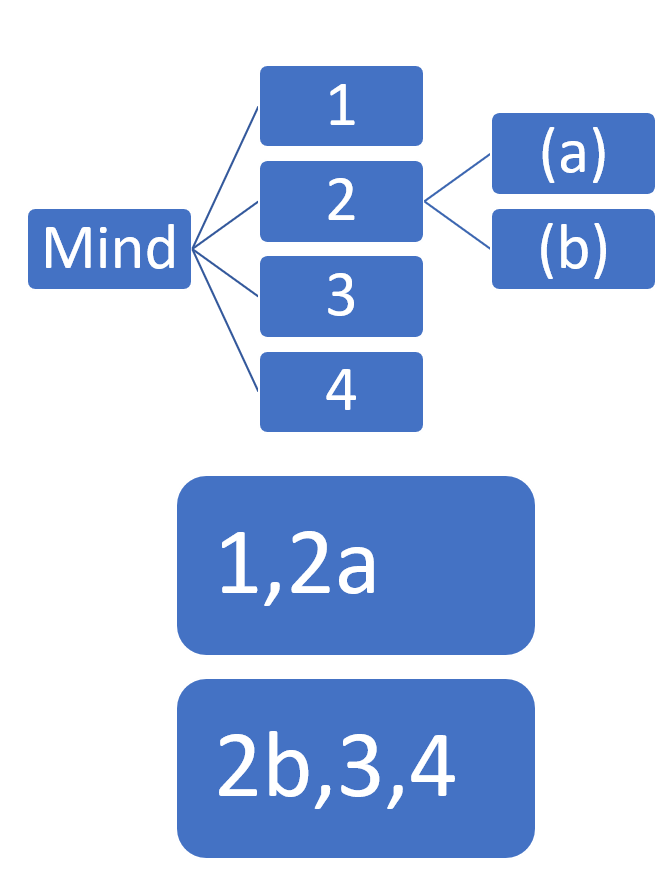
\includegraphics[width=0.9\linewidth,keepaspectratio]{images/zenyoga1}
\end{center}

\end{column}%
\end{columns}
\end{frame}

%%%%%%%%%%%%%%%%%%%%%%%%%%%%%%%%%%%%%%%%%%%%%%%%%%%%%%%%%%%%%%%%
\begin{frame}[fragile]\frametitle{}
\begin{center}
{\Large Notes from Other References}
\end{center}
\end{frame}


%%%%%%%%%%%%%%%%%%%%%%%%%%%%%%%%%%%%%%%%%%%%%%%%%%%%%%%%%%%%%%%%
\begin{frame}[fragile]
\frametitle{Mr.Deepak Dhingra}

``Introduction To Three Step Rhythmic Breathing(3SRB)''

\begin{itemize}
\item Death is a technical impossibility
\item We have no control internally. Many centers are producing impulses. Most of the organ functioning is autonomous
\item Thus we cannot control mind, but we have to bring them to rhythm, balance.
\item As per Pantanjali, daily, out of 13k impulses 120 go to brain. Rest are used to keep system working. Out of 120 to brain, 12 are per second, Only one becomes a thought. This just one more theory. May ignore. Just a model.
\item We are interpreting life our way and not how it is
\end{itemize}
\end{frame}

%%%%%%%%%%%%%%%%%%%%%%%%%%%%%%%%%%%%%%%%%%%%%%%%%%%%%%%%%%%%%%%%
\begin{frame}[fragile]
\frametitle{Introduction To Three Step Rhythmic Breathing(3SRB) By Mr.Deepak Dhingra}

Rhythmic Breathing and Refining exercises (6) for rhythm and balance

\begin{itemize}
\item In 3 sec out 2 sec | one hand chest one hand on belly| equal volume
\item  Same but with deep breathing
\end{itemize}
\end{frame}

%%%%%%%%%%%%%%%%%%%%%%%%%%%%%%%%%%%%%%%%%%%%%%%%%%%%%%%%%%%%%%%%
\begin{frame}[fragile]
\frametitle{Summary To-Dos}
\begin{itemize}
\item Breath: Three Step Rhythmic Breathing (book on tummy)
\item Food: lessen intake slowly to 1 time, be aware, get rid off addiction
\item Drift: Watch thoughts-wavering, Put in Fear/Anger/Sex/Hope/Jealousy
\item Walking with Awareness: 
\item Corrective methods: replace negative with positive thoughts
\item Sleep: 11 pm to 5 am. Other times do 3 step breathing
\item Reading
\item Sex Moderation
\item Awareness of Eyes: watch carefully, focus
\item Awareness of Ears: listen carefully, don't drift
\end{itemize}
\end{frame}
